\documentclass[14pt]{article}
\usepackage{graphicx}

\title{Tugas 2 Robust Control : Uncertainty }
\author{Donny Prakarsa Utama\\ \texttt{3332170032}
\and Ringga Dwi Raju\\ \texttt{3332170029} }
\maketitle

\begin{document}   
Mencari fungsi pembobotan $W(s)$ pada sistem uncertainty

1. $G(s)=\frac{1}{s+1}e^{-\theta s} ,\theta \in [0,0.1]$\\
Jawab :
Uncertainty pada soal ini hanya ada pada delay $ \theta $, dan dapat dibentuk menjadi $G(s)=\frac{e^{-\theta s}}{s+1}$ maka ditulis pada MATLAB
\begin{verbatim}
    exptheta =  ureal('exptheta',1.0526,'PlusMinus',[-0.0526,0.0526]);
\end{verbatim}
Kemudian buat fungsi alih nya menjadi
\begin{verbatim}
    sys = tf(exptheta ,[1 1])
\end{verbatim} 
Untuk pembobotan manual $W(s)$ didapat 
\begin{verbatim}
    W = tf([1],[0.8 0.8]) 
    bode(sys, 'b' , sys.NominalValue ,'r', W, 'g')
\end{verbatim}\\
Hasil dari bodeplot ada di Figure 1
\begin{figure}[hp]
    \centering
    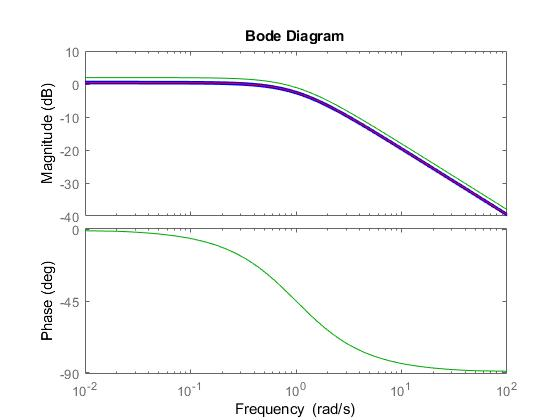
\includegraphics[width=79mm]{bodemanual1.jpg}
    \caption{$W(s)$ pembobotan manual \label{overflow}}
\end{figure}


2. $G(s)=\frac{1}{T_{1}s+1}.\frac{1}{T_{2}s+1} ,T_{1} \in [0,0.2], T_{2} \in [2,2.5]$ \\

Jawab : ada 2 Uncertainty yaitu $T_{Slow}$ dan $T_{Fast}$, dan fungsi alih dapat dibentuk menjadi $ \frac{1}{T_{1}T{2}s^2 + (T_{1}+T_{2})s + 1}$
\begin{verbatim}
    t1 = ureal('t1', 0.1, 'PlusMinus',[-0.1,0.1]);
    t2 = ureal('t2', 2.25 ,'PlusMinus',[-0.25,0.25]);
    sys = tf([1],[t1*t2 t1+t2 1])
\end{verbatim}

3. $G(s)=\frac{1}{s+1}.\frac{\omega^2}{s^2+2\zeta\omega s+\omega^2},\zeta \in [0.1,0.2],\omega\in[90,110]$\\
Jawab : ada 2 uncertainty yaitu $\zeta$ dan $\omega$ fungsi alih dapat dibentuk menjadi $   \frac{\omega ^2}{s^3+(2 \zeta   \omega +1)s^2+(2 \zeta   \omega + \omega ^2)s+\omega ^2} $
\begin{verbatim}
    w = ureal ('w', 100, 'PlusMinus',[-10,10]);
    z = ureal ('z',0.15 , 'PlusMinus',[-0.05,0.05]);
    sys= tf([w^2],[1 2*z*w+1 2*z*w+w^2 w^2])
\end{verbatim}

\end{document}